\documentclass[border=10pt]{standalone}

\usepackage{tikz}
\usepackage{tikzsymbols}
\usetikzlibrary{calc,patterns,shapes.geometric}

\def\centerarc[#1](#2)(#3:#4:#5){\draw[#1] ($(#2)+({#5*cos(#3)},{#5*sin(#3)})$) arc (#3:#4:#5);}

\begin{document}
	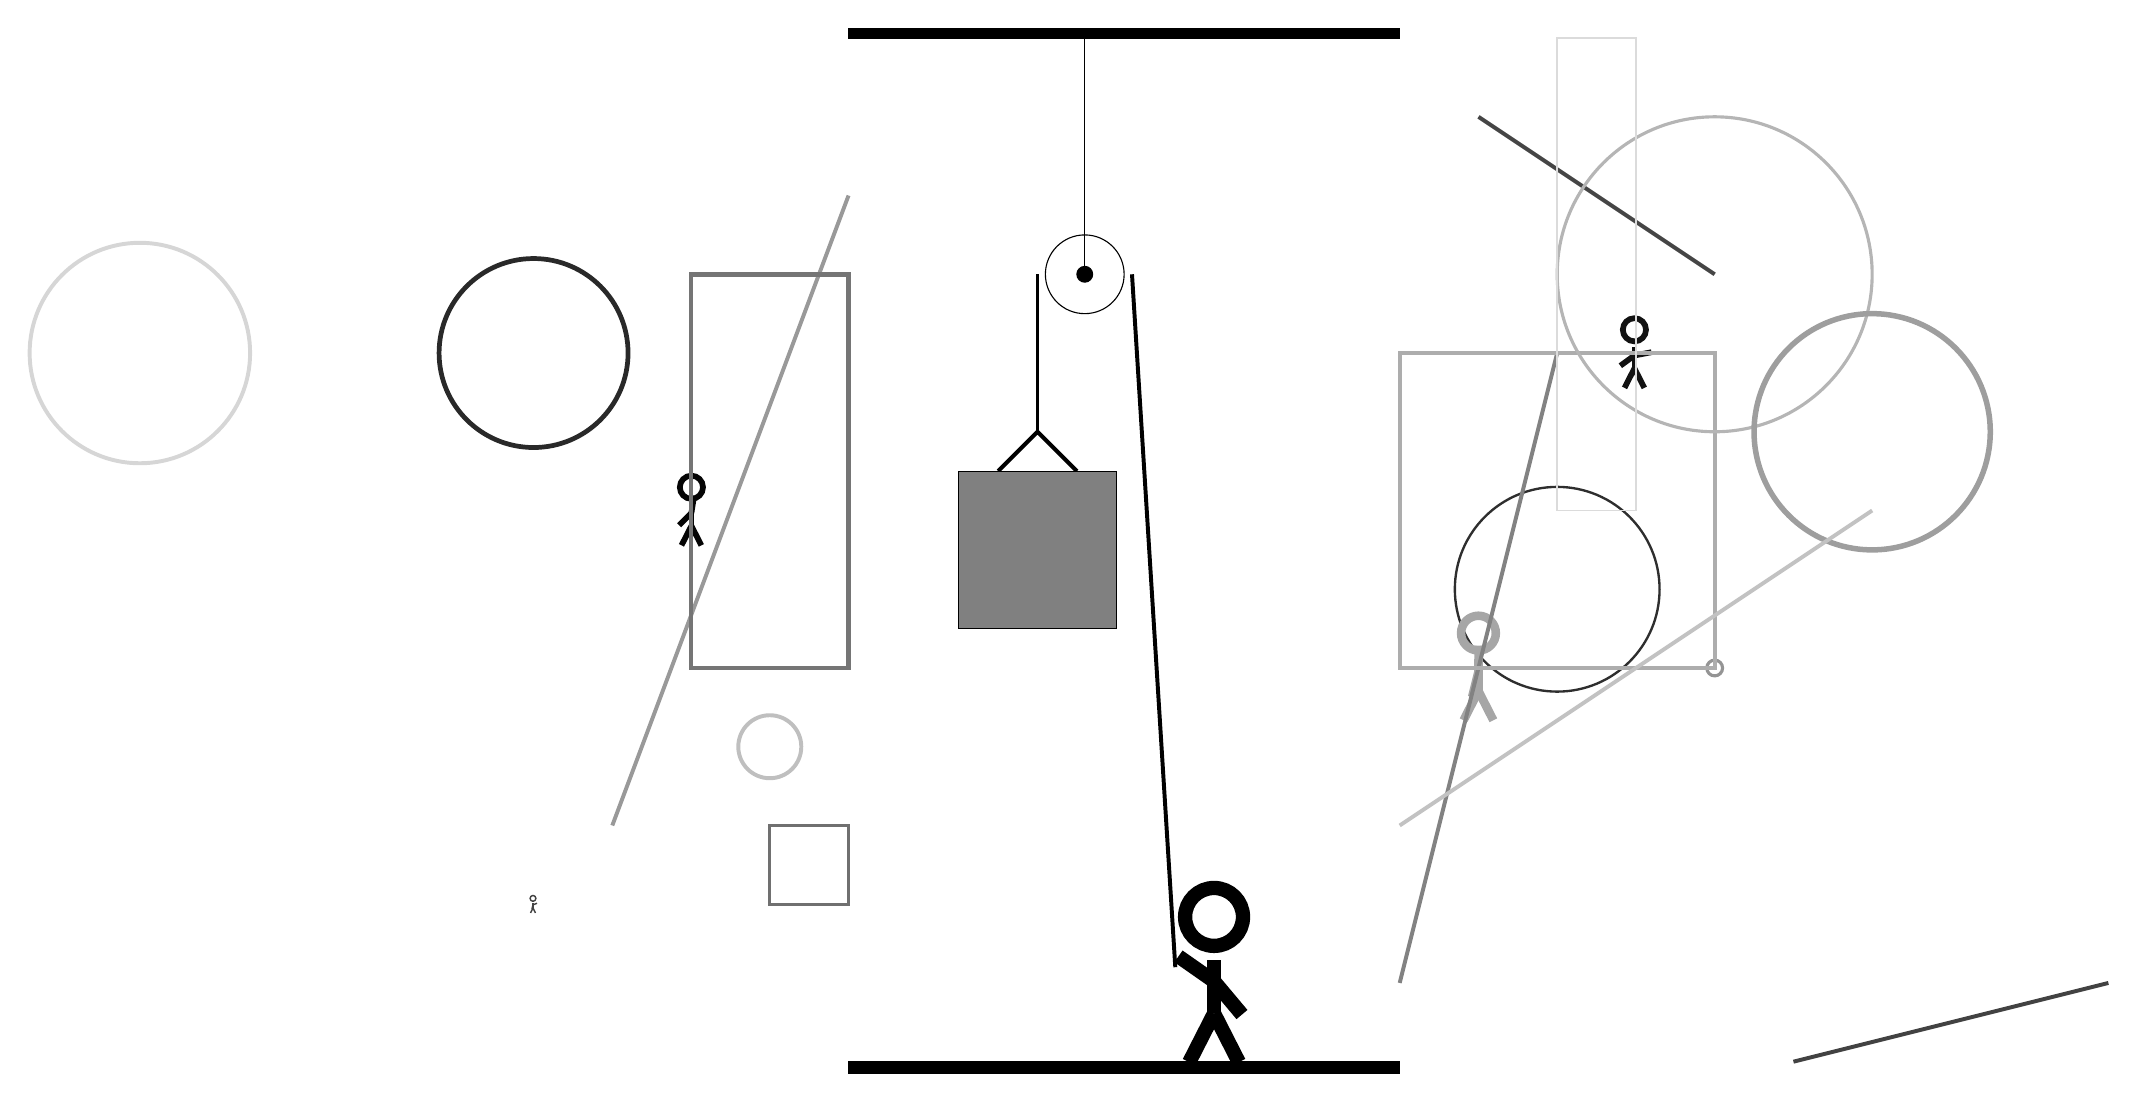
\begin{tikzpicture}
		%%%%% START %%%%%
		
		\draw[fill=black] (-2, 10) rectangle (5, 10.125);
		
		\node[line width=0.7mm, color=black!98] at (-4, 4) {\Strichmaxerl[4][45][81]};
		
		\draw [line width=0.5mm, color=black!16](-11, 6) circle (1.4);
		\draw [line width=0.3mm, color=black!82](7, 3) circle (1.3);
		\draw [line width=0.5mm, color=black!25](-3, 1) circle (0.4);
		\draw[line width=0.5mm, color=black!74](10, -3) -- (14, -2);
		
		\draw[line width=0.5mm, color=black!40](-2, 8) -- (-5, 0);
		
		\node[line width=0.5mm, color=black!35] at (6, 2) {\Strichmaxerl[6][76][89]};
		\draw[line width=0.5mm, color=black!49](7, 6) -- (5, -2);
		\draw[line width=0.4mm, color=black!56] (-2, 0) rectangle (-3, -1);
		
		\draw[line width=0.5mm, color=black!73](9, 7) -- (6, 9);
		
		\node[line width=0.6mm, color=black!93] at (8, 6) {\Strichmaxerl[4][36][11]};
		\node[line width=0.2mm, color=black!74] at (-6, -1) {\Strichmaxerl[1][76][21]};
		\draw[line width=0.6mm, color=black!54] (-4, 2) rectangle (-2, 7);
		
		\draw [line width=0.6mm, color=black!84](-6, 6) circle (1.2);
		\draw [line width=0.4mm, color=black!42](9, 2) circle (0.1);
		\draw[line width=0.5mm, color=black!32] (5, 6) rectangle (9, 2);
		\draw [line width=0.4mm, color=black!29](9, 7) circle (2.0);
		
		\draw[line width=0.2mm, color=black!14] (7, 10) rectangle (8, 4);
		\draw [line width=0.7mm, color=black!38](11, 5) circle (1.5);
		\draw[line width=0.5mm, color=black!24](5, 0) -- (11, 4);
		
		\draw (1, 7) circle (0.5);
		\draw[fill=black] (1, 7) circle (0.1);
		\draw (1, 10) -- (1, 7);
		
		\draw[line width=0.5mm] (-0.1, 4.5) -- (0.4, 5.0) -- (0.9, 4.5);
		\draw[fill=black!50] (-0.6, 4.5) rectangle (1.4, 2.5);
		
		\draw[line width=0.5mm] (0.4, 7) -- (0.4, 5.0);
		\centerarc[line width=0.5mm](1, 7)(0:180:0.6);
		\draw[line width=0.5mm](1.6, 7) -- (2.15, -1.8);
		
		\node at (2.6, -1.9) {\Strichmaxerl[10][-35][-50]};
		
		\draw[fill=black] (-2, -3) rectangle (5, -3.15);
		
		%%%%% END %%%%%
	\end{tikzpicture}
\end{document}